\section{Description des mises en situation}
\begin{itemize}
    \item \textbf{\textcolor{green}{[A1]}} Constitution du groupe durant la séance de TD7.
    \item \textbf{\textcolor{green}{[A2]}} On peut trouver notre repository git \href{https://github.com/jortanix/gestion_projet/branches}{ici}.
    
    \item \textbf{\textcolor{green}{[A3]}} Git status
    \begin{figure}[H]
        \centering
        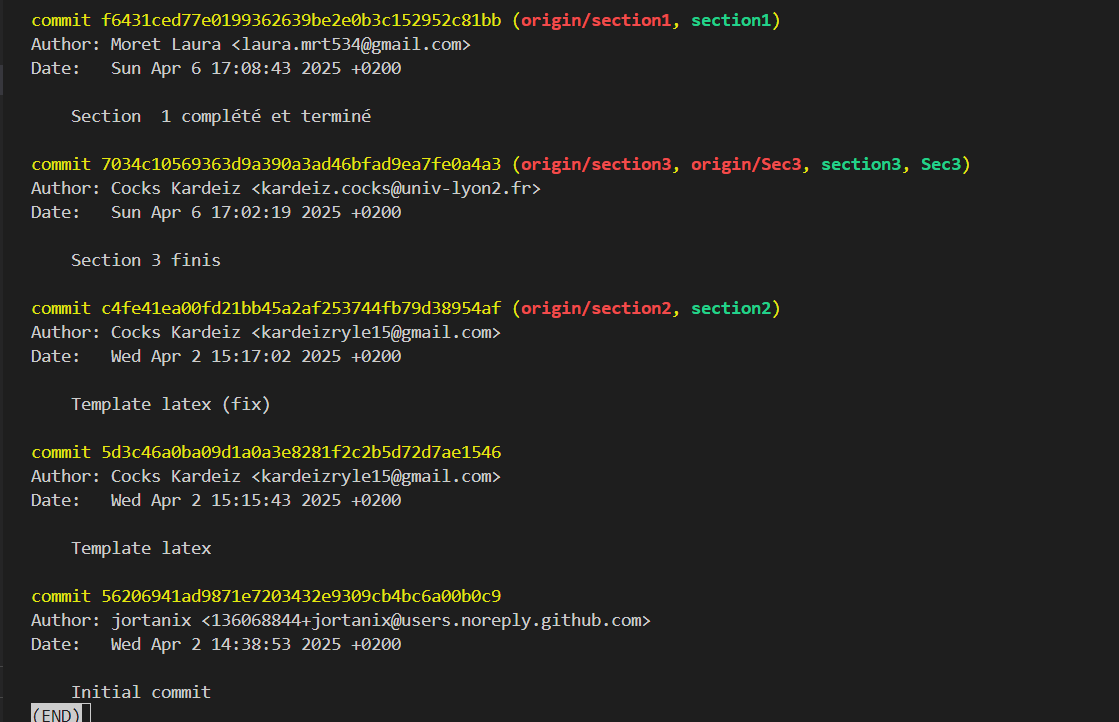
\includegraphics[width=0.8\linewidth]{Images/A3.png}
        \caption{Capture de l'historique des commits}
        \label{fig:imageA3}
    \end{figure}
    
    \item \textbf{\textcolor{orange}{[B1]}} Nous avons décidé d'utilisé différentes branches pour les commits des différentes sections du fichiers latex.
    
    \begin{figure}[H]
    \centering
    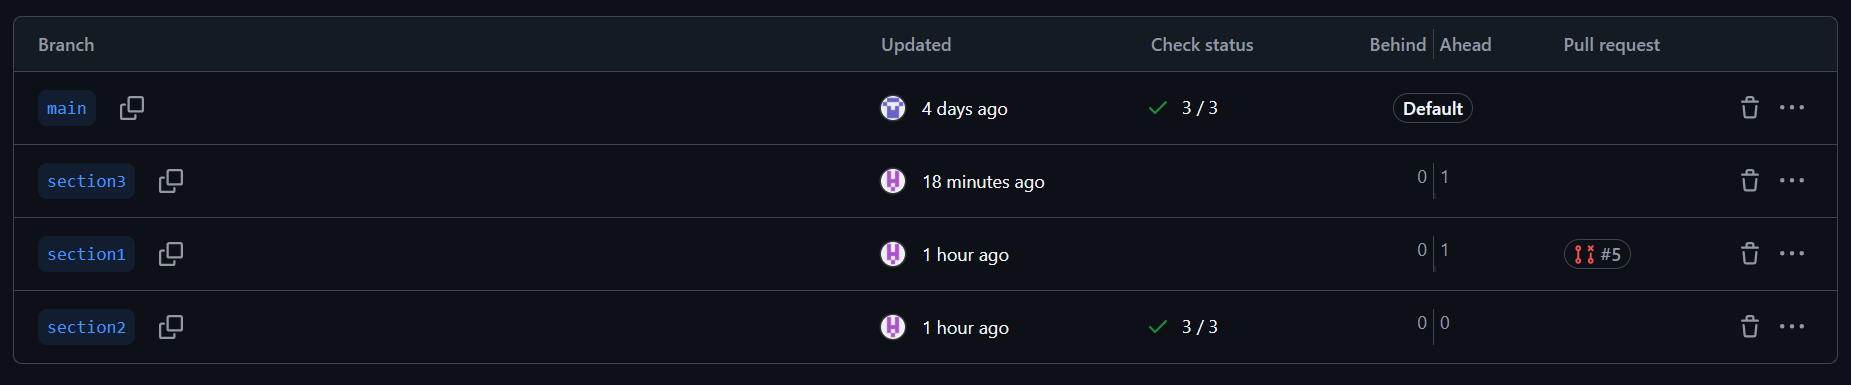
\includegraphics[width=0.8\textwidth]{Images/B1.png}
    \caption{Capture des branches}
    \label{fig:imageB1}
    \end{figure}
    
    \item \textbf{\textcolor{orange}{[B2]}} Création d'une version Contenant la Section 1 et Section 3.
    \begin{figure}[H]
    \centering
    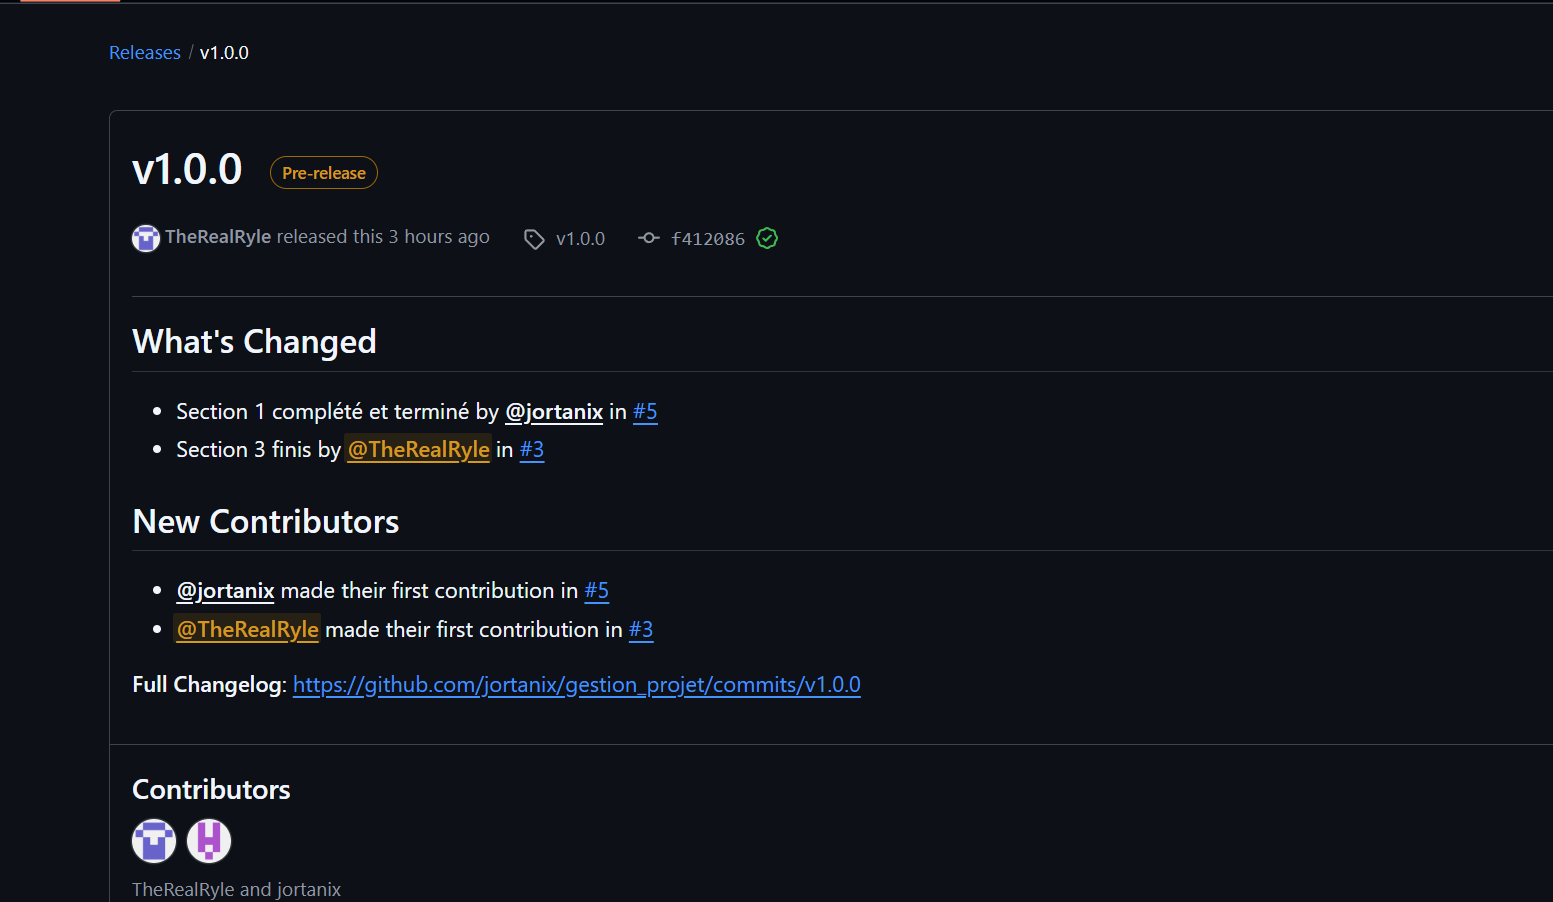
\includegraphics[width=0.8\textwidth]{Images/B2.png}
    \caption{Capture}
    \label{fig:imageB2}
    \end{figure}
    
    \item \textbf{\textcolor{orange}{[B3]}} Pull request pour intégrer la Section 1 (Introduction), la branche Section 1 sera ensuite merger.
    \begin{figure}[H]
    \centering
    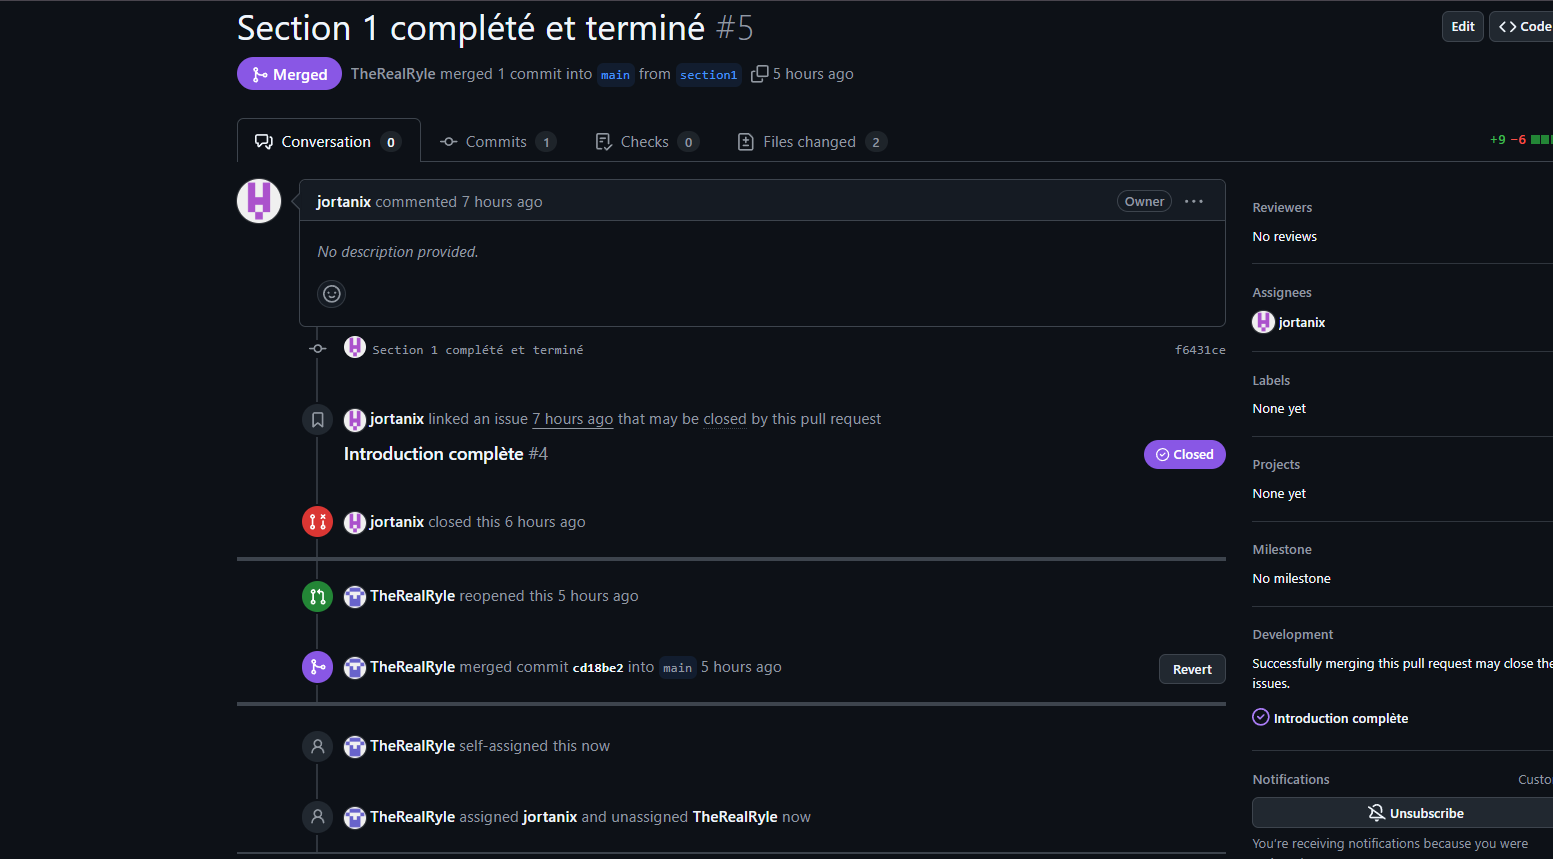
\includegraphics[width=0.8\textwidth]{Images/B3.png}
    \caption{Capture des Pull Requests}
    \label{fig:imageB3}
    \end{figure}

    
    \item \textbf{\textcolor{orange}{[B4]}}
    \item \textbf{\textcolor{red}{[C1]}} Les milestones du projet nous permettent de savoir où on en est dans le projet.
    \begin{figure}[H]
    \centering
    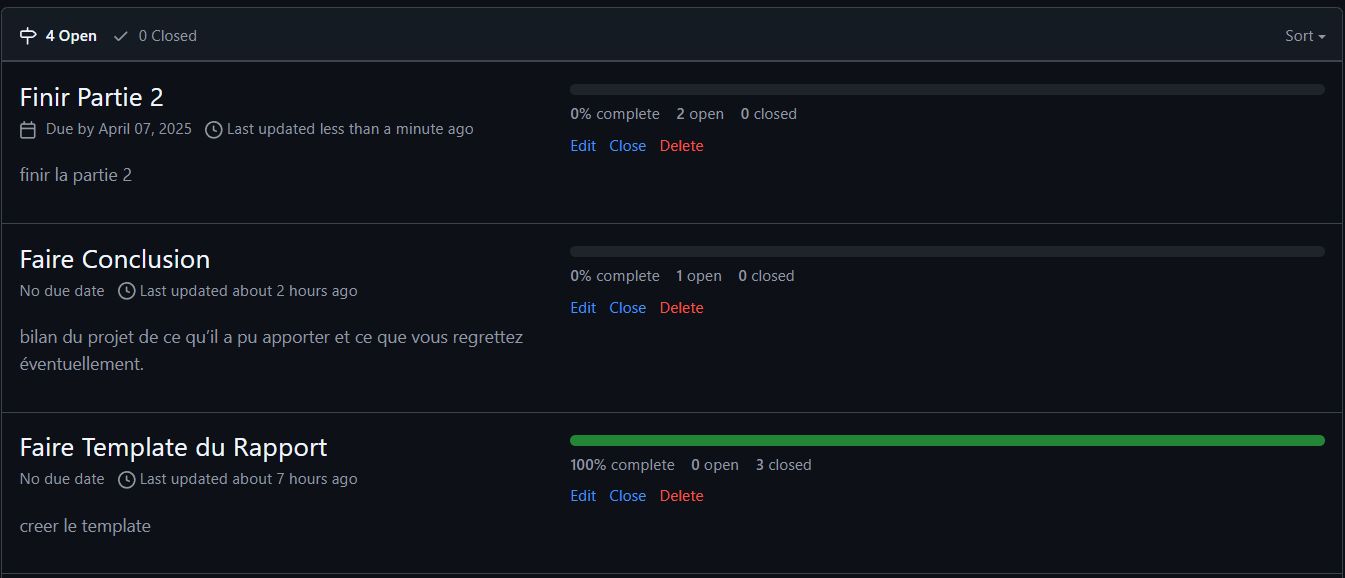
\includegraphics[width=0.8\textwidth]{Images/C1.png}
    \caption{Capture des milestones}
    \label{fig:imageC1}
    \end{figure}

\end{itemize}